\documentclass{article}
\usepackage{setspace}
\usepackage[text={6.5in,8.5in},centering]{geometry}
\geometry{verbose,a4paper,tmargin=2.4cm,bmargin=2.4cm,lmargin=2.4cm,rmargin=2.4cm}
\usepackage{graphicx,amsmath,cases,multirow,appendix,graphicx,xcolor,cancel,tikz}

\setlength\parindent{0pt}

\newcommand{\note}[1]{\colorbox{gray!30}{#1}}
\newcommand{\ind}{\-\hspace{1cm}}
\newcommand*\circled[1]{\tikz[baseline=(char.base)]{
            \node[shape=circle,draw,inner sep=2pt] (char) {#1};}}


\begin{document}

\noindent\makebox[\textwidth][c]{\Large\bfseries Lecture 7 -- Model-fitting - Maximum Likelihood and AIC}

\rule[0.5ex]{\linewidth}{1pt}
\textbf{Announcements}:
\ind Today: lecture \& paper discussion\\
\ind Next time: Bring laptops! (Playing with chaos)\\
\textbf{Concepts}: 
\ind Maximum likelihood \& AIC\\
\rule[0.5ex]{\linewidth}{1pt}
Recall that least squares estimates of parameters are ``most likely'' values given the data:\\
\begin{equation*}
	\mathcal{L}(\beta \vert Y) \quad \quad \text{sometimes} \quad \mathcal{L}(\vec{\beta} \vert \vec{Y})
\end{equation*}
\ind $\beta$ = (vector of) parameters\\
\ind $y$ = (vector of) data\\

Likelihood of a particular parameter value, $\beta$, given a data point $y_i$ is proportional to the probability of observing $y_i$ given that $\beta$ is true.
\begin{equation*}
	\mathcal{L}(\beta \vert y_i) \propto P(y_i\vert \beta)
\end{equation*}

Thus, if the data $Y$ are described by a particular distribution (e.g., Binomial, Poisson, Normal), we can quantify the likelihood using the probability of that distribution (or probability density function).\\

Example:  Poisson whales\\
Poisson describes freq. of rare events with a single parameter, $\lambda$.\\
\ind (e.g., encountering a whale on an ocean transect)
\begin{align*}
	P(x \vert\lambda) & = \frac{\lambda^x e^{-\lambda}}{x!} \quad x=0,1,2,... & \text{Probability distribution}\\
	\mathcal{L}(\lambda \vert x) & = \prod_{i=1}^n P(x_i\vert \lambda) = \prod_{i=1}^{n}\frac{\lambda^{x_i}e^{-\lambda}}{x_i !} & \text{Likelihood function}
\end{align*}
Say we see 4 whales in one transect...
What is the likelihood of a given value of $\lambda$?
\begin{equation*}
	\mathcal{L}(\lambda \vert 4) = P(4 \vert \lambda) = \frac{e^{-\lambda}\lambda^4}{4!}
\end{equation*}
$\lambda$ = ``encounter rate''\\

Evaluate over all possible values of $\lambda$.\\
The value that \emph{maximizes} $P(4\vert \lambda)$ is the MLE of $\lambda$ $\Rightarrow$  
	MLE of $\lambda = max. \mathcal{L}(\lambda \vert y_i)$\\
\note{Show R plot}
\begin{center}
	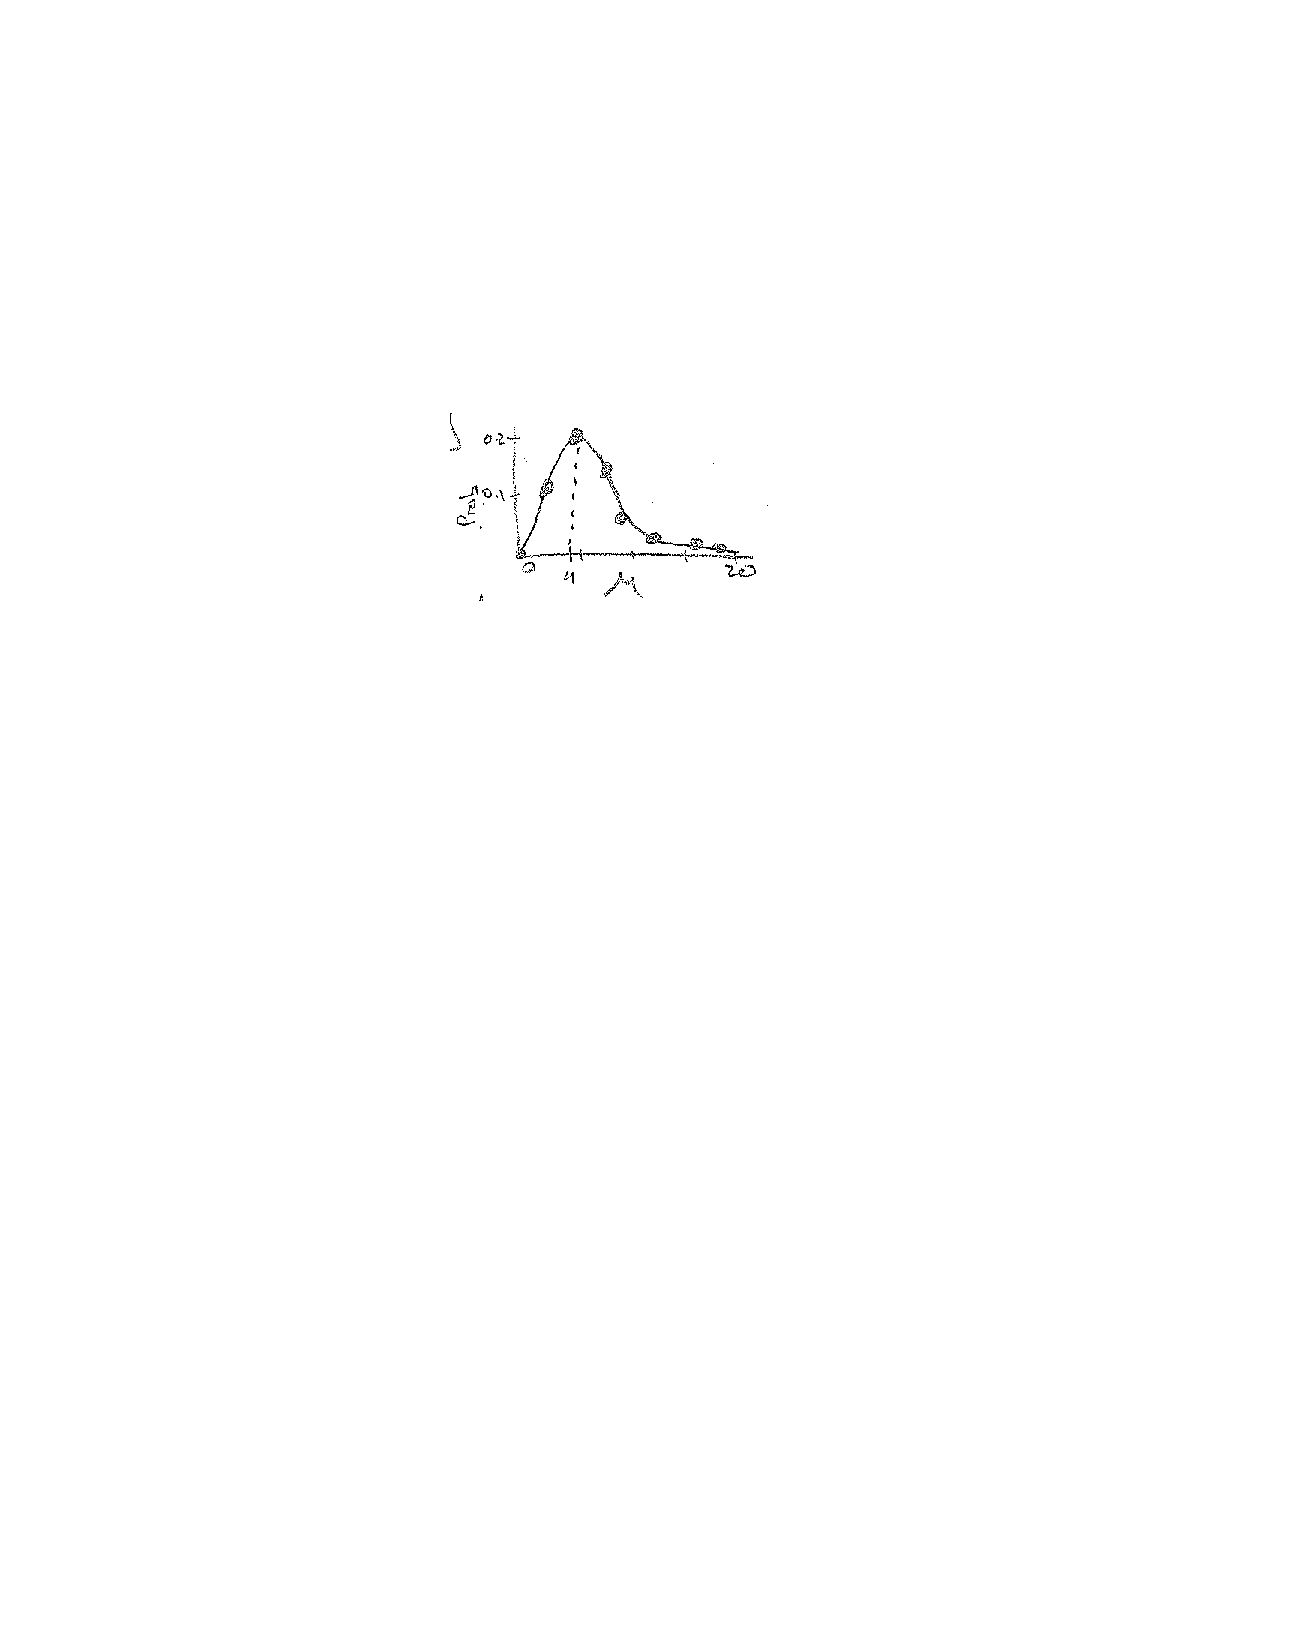
\includegraphics[width=5cm]{figs/image5.pdf}
\end{center}
...shows that MLE of encounter rate = 4 per transect\\
\ind (not surprising given 4 whales encountered in 1 transect)\\

Perform 2nd transect, observe 6 whales.  But $P(y_i=6 \vert \lambda=4)=0.1$ only (low probability).\\

Therefore:  \emph{Joint probability}!\\

Joint probability of two independent events is the product of their probabilities.
\begin{equation*}
	P(A \cap B) = P(A) \cdot P(B)
\end{equation*}
Therefore:
\begin{equation*}
	\mathcal{L}(\lambda \vert [4,6]) = \mathcal{L}(\lambda \vert 4) \cdot \mathcal{L}(\lambda \vert 6)
\end{equation*}
Again, evaluate over all possible $\lambda$ values...\\
\note{Show R plot}
\begin{center}
	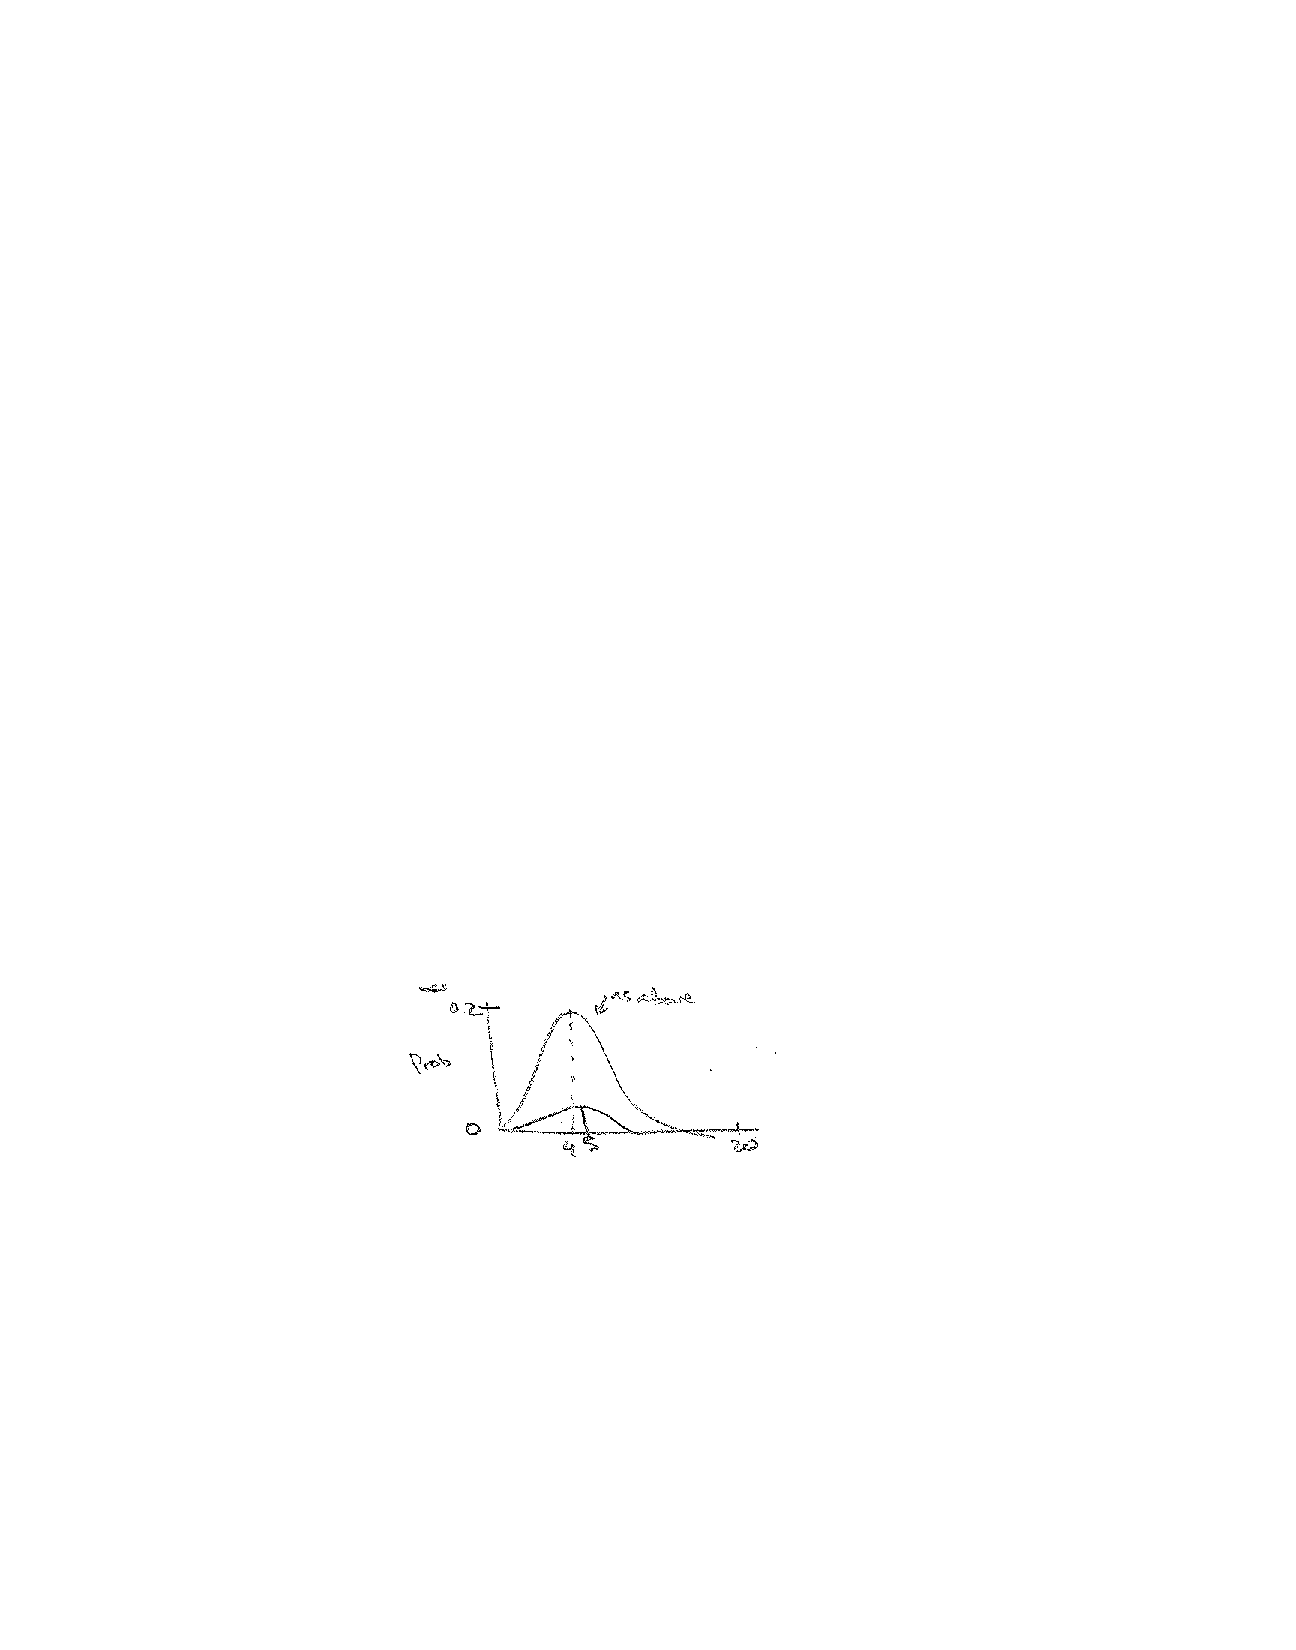
\includegraphics[width=5cm]{figs/image6.pdf}
\end{center}
...shows that MLE of encounter rate = 5 per transect\\

But notice that joint probability declines with each additional observation!
\begin{equation*}
	\mathcal{L}(\lambda \vert y_i) \propto \prod P(y_i \vert \lambda)
\end{equation*}
Therefore take log...
\begin{center}
	Log(small number) = negative normal-sized number
\end{center}
Therefore take negative log...
That's why we use \emph{Negative Log Likelihood} (NLL)
\begin{equation*}
	-\ln \mathcal{L}(\lambda \vert y_i) \propto \sum_i^n -\ln( P(y_i \vert \lambda))
\end{equation*}
Because we've taken the negative $\Rightarrow$ Value that \emph{minimizes} NLL is the MLE.\\

How to find MLE of parameter analytically?\\
\note{Class Q:}  How does one find the min or max of a function?\\
\ind \note{A:} Take derivative with respect to focal parameter, set to zero, solve!

\rule[0.5ex]{\linewidth}{1pt}
\textbf{Back to Popn Growth data}\\
Assume process-error only.\\
\ind Process model: 
\begin{equation*}
	N_{t+1} = F(N_t)
\end{equation*}
Assume $log\mathcal{N}$ residual error distribution, thus...
\begin{align*}
	\ln \left(\frac{N_{t+1}}{N_t}\right) &= \ln \left(\frac{F(N_t)}{N_t}\right) + \epsilon_t\\
	\epsilon_t &\sim \mathcal{N}(\mu,\sigma^2)
\end{align*}

For Normal distribution:
\begin{align*}
	f(y\mid \mu,\sigma) & =\frac{1}{\sqrt{2 \pi \sigma^2}} \exp \frac{-(y-\mu)^2}{2\sigma^2} \quad \quad \text{Probability density function}\\
	-\ln \mathcal{L}(\mu, \sigma \mid Y) &=   \frac{n}{2} \ln \left(2 \pi \sigma^2 \right) + \frac{1}{2\sigma^2}\sum_{i=1}^n (y_i - \mu)^2
\end{align*}
In our context of model-fitting
\begin{equation*}
	-\ln \mathcal{L}(\beta \mid Y) =   \frac{n}{2} \ln \left(2 \pi \sigma_y^2 \right) + \frac{1}{2 \sigma_y^2}  \sum_{t=1}^n (obs.growth_t- pred.growth_t)^2
\end{equation*}
where
\begin{align*}
	y_t &= \ln\left(\frac{N_{t+1}}{N_t}\right)\\
	\sigma_y^2  &= \frac{1}{n-1} \sum_t^n (y_t - \bar{y})^2 \quad \text{=Variance of observed growth rates}
\end{align*}

Remember: The MLE of $\epsilon_t \sim \mathcal{N}(\mu,\sigma^2)$ = least squares estimate.\\
\ind  Thus in R we can thus use $lm$ (linear least squares) or $nls$ nonlinear least squares.\\

\rule[0.5ex]{\linewidth}{1pt}
\pagebreak

\textbf{Model comparison}\\
\note{R-exercise} Great tit dataset (setup for models used in PS3)
\begin{center}
	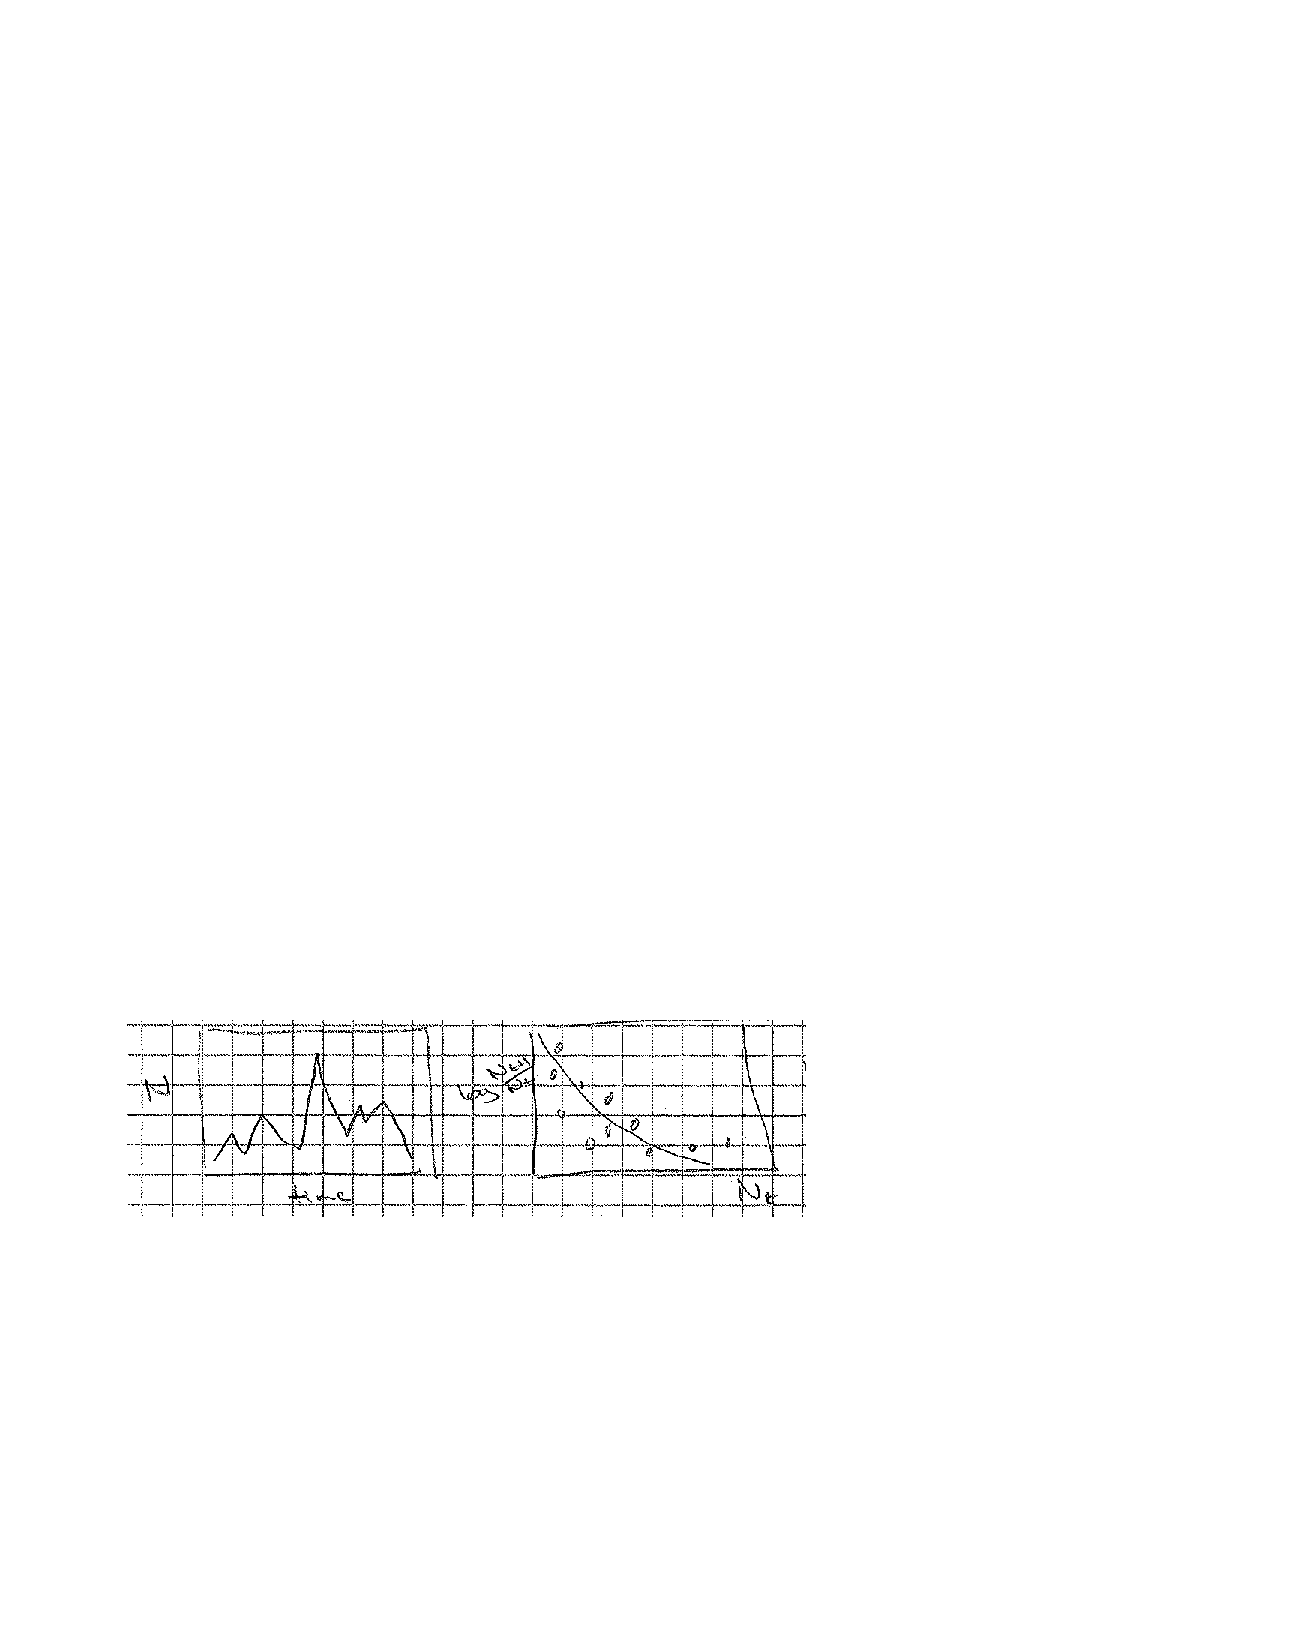
\includegraphics[width=12cm]{figs/image7.pdf} Note curvature!
\end{center}


Three hypothesized models:\\
\begin{tabular}{|c|c|c|}
\hline
   & $N_{t+1}$ & $\ln \left(\frac{N_{t+1}}{N_t} \right)$ \\ 
 \hline
Density-independent & $N_t e^r$ & $r$ \\ 
Ricker (linear DD) & $N_t e^{r(1-N/K)}$ & $r\left(1-\frac{N}{K}\right)$ \\
Theta-logistic (nonlinear DD) & $N_t e^{r(1-N/K)^\theta}$ & $r\left(1-\frac{N}{K}\right)^\theta$ \\
\hline
\end{tabular}
Note:  Implicitly using $e^{r\cdot 1}$ since $\Delta t = 1$\\
\begin{center}
	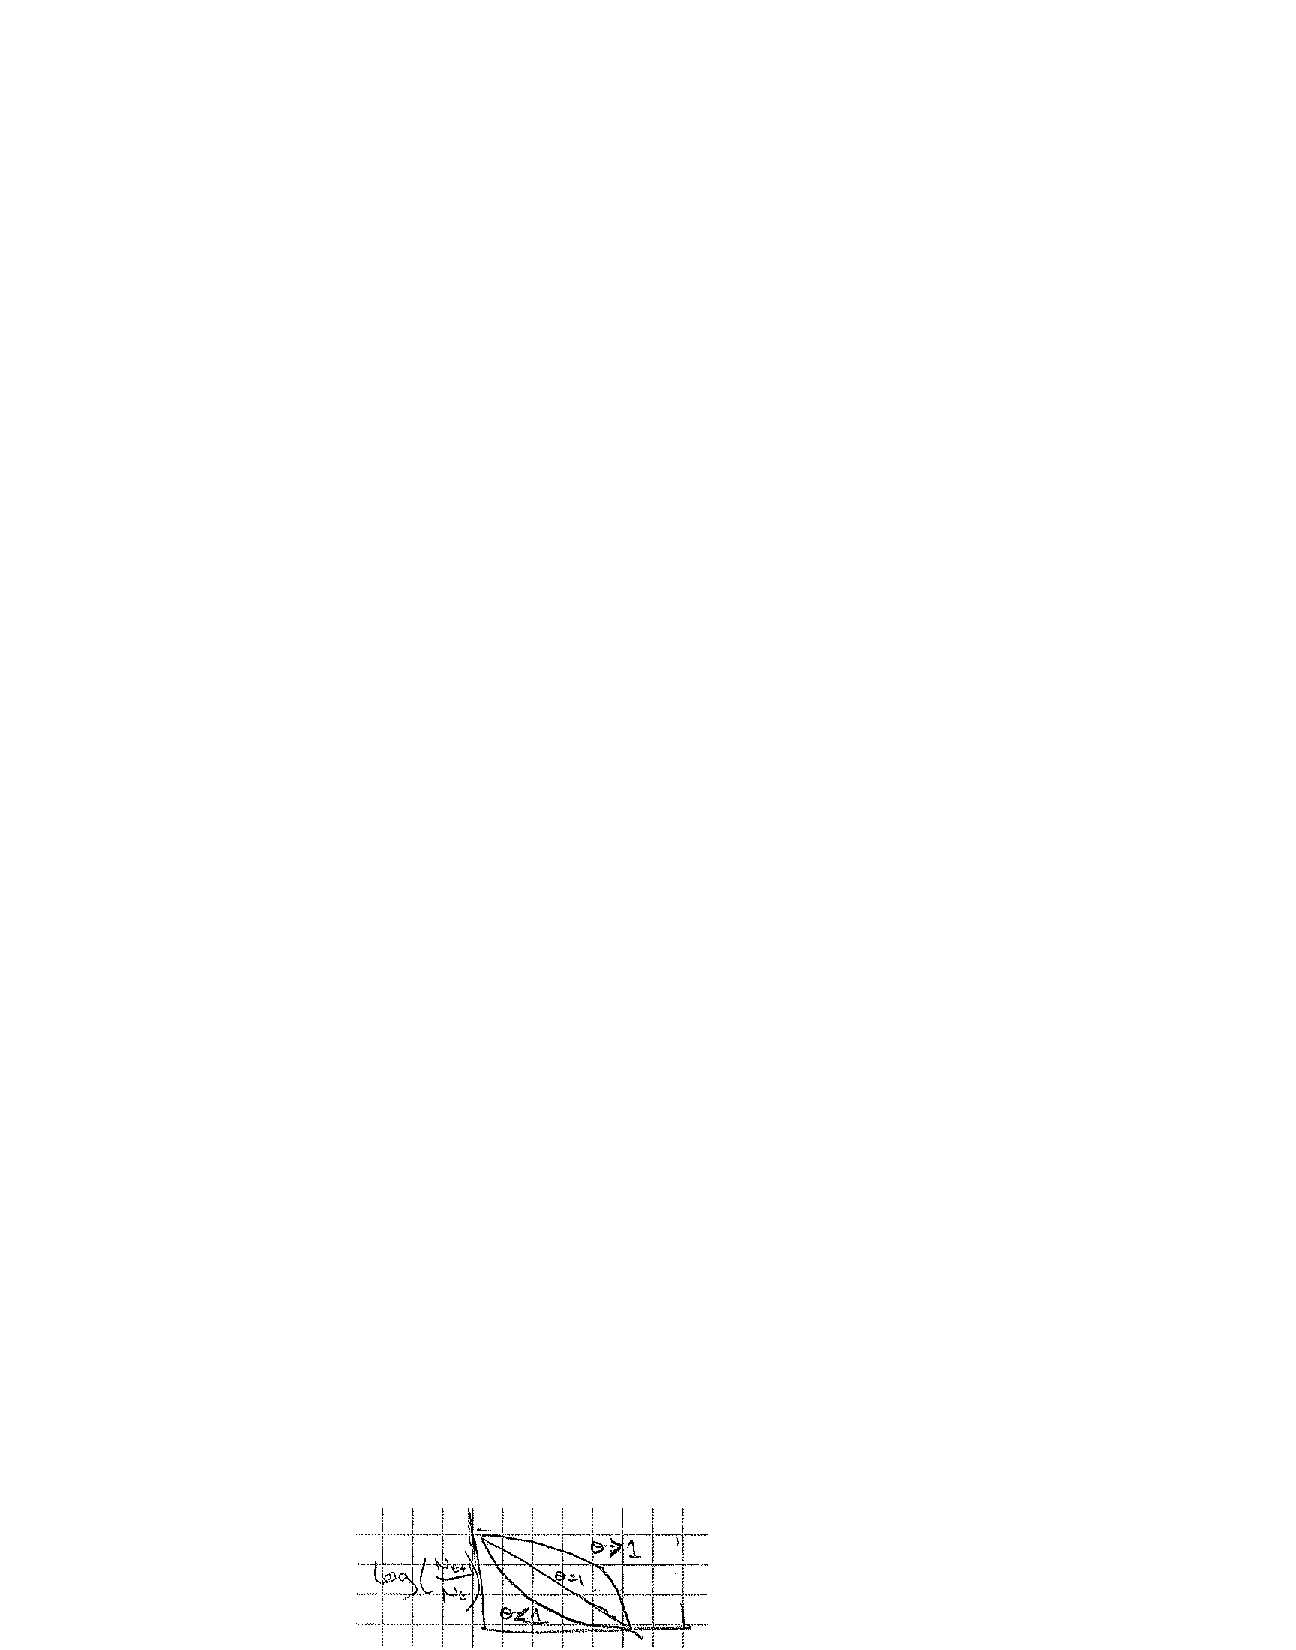
\includegraphics[width=7cm]{figs/image8.pdf}
\end{center}

\note{Aside:  Advise against using Theta-logistic.  Has conceptual problems.  Use in PS3  for illustrative purposes.}\\

For each model, plug in predicted values for each time step into NLL eqn.\\

\begin{tabular}{|c|c|}
\hline
   & NLL \\ 
 \hline
Density-independent & 22.526 \\ 
Ricker (linear DD) & 14.299 \\
Theta-logistic (nonlinear DD) & 14.058 \\
\hline
\end{tabular}
\ind $\Rightarrow$ Theta-logistic fits best!\\


So is Theta-logistic the best model?\\
\ind ``Best fit'', but ``best-performing''???  Remember polynomial from first class!\\

$\Rightarrow$ Akaike Information Criterion (AIC)\\
\ind Penalize models for number of parameters ($p$) [Note: don't forget $\sigma$ for normal!]
\begin{equation*}
	\text{AIC} = 2p - 2\cdot \ln(\mathcal{L}_{\text{MLE}}) = 2 \cdot \text{NLL}_{\text{MLE}} + 2p
\end{equation*}
Small sample size correction:
\begin{equation*}
	\text{AIC}_c = 2 \cdot \text{NLL}_{\text{MLE}} + 2p \left(\frac{n}{n-p-1}\right)
\end{equation*}
\ind where $n$ is number of data points.\\

Model with lowest AIC is the ``best-performing'' model.\\
Typically given using $\Delta$AIC of $i$th model:
\begin{equation*}
\Delta \text{AIC}_i = \text{AIC}_i - min(\text{AIC})
\end{equation*}

Relative likelihood of models - Akaike weights:\\
``Probability of model given the data''
\begin{equation*}
	w_i = \frac{e^{-\frac{1}{2} \Delta \text{AIC}_i}}{\sum_k e^{-\frac{1}{2} \Delta \text{AIC}_k}}
\end{equation*}

%\begin{tabular}{|c|c|c|c|c|c|c|}
%\hline
%   & NLL & p & AIC & AICc & $\Delta$AICc & w \\ 
% \hline
%Density-independent & 22.526 & 1 & 47.05 & 47.2 & 14.14 & 0.006 \\ 
%Ricker (linear DD) & 14.299 & 2 & 32.60 & 33.06 & 0 & 0.73 \\
%Theta-logistic (nonlinear DD) & 14.058 & 3 & 34.12 & 35.08 & 2.02 & 0.27\\
%\hline
%\end{tabular}

\rule[0.5ex]{\linewidth}{1pt}
\textbf{Paper discussion}\\
\rule[0.5ex]{\linewidth}{1pt}

\pagebreak

\textbf{Extra: Continuous probability functions vs. discrete probability distributions}

Q: Why do I sometimes write
\begin{equation*}
	\mathcal{L}(\beta \mid Y) \propto P(Y  \mid \beta),
\end{equation*}
and other times
\begin{equation*}
	\mathcal{L}(\beta \mid Y)= P(Y  \mid \beta)
\end{equation*}
It turns out that both are in some ways correct!  There are two relevant distinctions:\\

Distinction 1: $\mathcal{L}(\beta \mid Y) \propto P(Y  \mid \beta)$ is correct for \emph{continuous} distributions while $\mathcal{L}(\beta \mid Y)= P(Y  \mid \beta)$ is correct for \emph{discrete} distributions.  The reason is that, unlike for a discrete distribution, the probability of any specific value on a continuous distribution is zero!  It's only over some interval of values that we can speak of a continuous distribution having some probability.\\

Distinction 2: However, the equality is still correct when the right hand side is not a \emph{probability distribution}, $P(Y \mid \beta)$, but rather a \emph{probability density function}, $f(Y \mid \beta)$.  These differ even though $\int f(Y \mid \beta) d\beta= \sum P(Y \mid \beta) = 1$ (i.e the total area under both equals 1).  Most people loosely (but technically incorrectly) use these two terms interchangeably. 

\rule[0.5ex]{\linewidth}{1pt}
\rule[0.5ex]{\linewidth}{1pt}

\end{document}